Detached from the noise model, the goal of image denoising is to estimate the true image $\mathbf{X}$ from the noisy observation $\mathbf{Y}$. Let $\mathbf{i} = [i_1, i_2, \dots, i_d]^T$ be a column vector that defines the coordinates of each voxel in a \textit{d}-dimensional image space. In the most general form, $\mathbf{Y_{\mathbf{i}}}$ is a mapping of $\mathbf{X_{\mathbf{i}}}$ through a function $\mathcal{F}$:
\begin{equation*}
    \mathbf{Y_{\mathbf{i}}} = \mathcal{F} (\mathbf{X_{\mathbf{i}}})
\end{equation*}
where $\mathbf{Y_{\mathbf{i}}}$ and $\mathbf{X_{\mathbf{i}}}$ represent the noisy observation and the corresponding true image value at voxel $\mathbf{i}$, respectively.

The inverse problem is then to estimate $\mathbf{X}$ from $\mathbf{Y}$ (denoising), which is an ill-posed problem, meaning that there are multiple possible solutions for $\mathbf{X}$ that could generate $\mathbf{Y}$.

Denoising of images has been explored in both the spatial and transform domains. In the spatial domain, various linear and non-linear filtering techniques can be seen that utilize different kernels to manipulate pixel values directly. Linear filters, such as the mean filter, compute the average of pixel values within a neighborhood, smoothing the image but often blurring edges. Non-linear filters, like the median filter, replace each pixel with the median value of its neighbors, making them particularly effective for removing salt-and-pepper noise while preserving edges. Wiener filtering is another example, operating on statistical principles. The \gls{MSE} between the estimated and true image is minimized, adjusting the filter response according to the local image variance. This makes Wiener filtering particularly effective for Gaussian noise, as it can adaptively filter based on the estimated noise level and the signal characteristics, often resulting in superior denoising performance compared to simpler linear methods. More advanced non-linear methods, such as bilateral filtering, combine spatial proximity and intensity similarity, allowing for selective smoothing that retains sharpness around edges.

In addition to these filtering techniques, many denoising methods leverage prior knowledge about image characteristics, which significantly enhances their effectiveness. Common priors include assumptions about sparsity, smoothness, and texture. For example, total variation (TV) denoising assumes that natural images exhibit piece-wise smoothness, enabling the algorithm to preserve edges while reducing noise in flat regions. This method minimizes the total variation of the image, resulting in a denoised image that maintains important structural information. Similarly, non-local means (NLM) denoising capitalizes on the redundancy of similar patches within the image, estimating the value of a pixel based on a weighted average of other pixels with similar local structures, regardless of their spatial distance. By employing these priors, denoising algorithms can effectively exploit the inherent properties of images, leading to improved visual quality and more accurate representations of the true scene. Overall, the combination of spatial and transform domain techniques, along with the integration of prior knowledge, forms a robust framework for tackling the challenges of image denoising.


\section{BM3D: Denoising in Sparse Domain}
A lot of the mentioned algorithm assume additive noise.
\begin{equation*}
    \mathbf{Y} = \mathbf{X} + \mathbf{N}
\end{equation*}
and many algorithms assume the noise to be \gls{AWGN}.

\begin{equation*}
    \mathbf{N} \sim \mathcal{N}(0, \sigma^2)
\end{equation*}

The celebrated \gls{BM3D} algorithm, introduced first by \citeauthor{dabovImageDenoisingSparse2007} in \cite{dabovImageDenoisingSparse2007}, builds upon many of the classical denoising techniques as seen above. The proposed scheme (see algorithm~\ref{alg:bm3d}) works by grouping similar patches in a 2D image and applying a 3D transform\footnote{This algorithm has also been proposed for 3D images, dubbed BM4D.}. This leads to an enhanced sparse representation of the image which after filtering is transformed back to the spatial domain.
% Main BM3D Algorithm
\begin{algorithm}
    \caption{BM3D Denoising Algorithm}\label{alg:bm3d}
    \begin{algorithmic}[1]
    \Require Noisy image $I$
    \Ensure Denoised image $I_{\text{denoised}}$
    \Statex
    \Procedure{BM3D}{$I$, $\sigma^2$, $b$, $W$, $\tau$}
        \State $I_{\text{denoised}} \gets I$
        
        \For{each reference block $B_r$ in $I$}
            \State $\mathcal{B} \gets \textsc{Grouping}(B_r)$
            \State $B_{\text{filtered}} \gets \textsc{CollaborativeFiltering}(\mathcal{B})$
            \State Aggregate $B_{\text{filtered}}$ into $I_{\text{denoised}}$
        \EndFor
        
        \State \textbf{return} $I_{\text{denoised}}$
    \EndProcedure
    \end{algorithmic}
\end{algorithm}

In the Grouping step, blocks who are the least dissimilar to the reference block $B_r$ are used. The dissimilarity measure used is the $l^2$-distance. The Collaborative Filtering\footnote{Interestingly, collaborative filtering has been the backbone of recommendation systems such as by Netflix and Spotify.} shown in Algorithm~\ref{alg:collaborativefiltering} is then applied to the grouped blocks. This step consists of a 3D transform such as the discrete cosine transform (or the wavelet transform can be used). A filter is applied to the transformed blocks to remove noise, initially by hard thresholding and in the second run by Wiener filtering. The inverse 3D transform is then applied to the filtered blocks, and the filtered blocks are aggregated to form the estimate. The first run is considered the basic estimate, and it is only after Collaborative Wiener filtering that the final estimate is obtained.
    
% Collaborative Filtering Algorithm
\begin{algorithm}
    \caption{Collaborative Filtering}\label{alg:collaborativefiltering}
    \begin{algorithmic}[1]
    \Require Group of similar blocks $\mathcal{B}$
    \Ensure Filtered block $B_{\text{filtered}}$
    \Procedure{CollaborativeFiltering}{$\mathcal{B}$}
        \State Apply 3D transform (e.g., DCT) to $\mathcal{B}$
        \State Apply filtering (hard thresholding or Wiener)
        \State Perform inverse 3D transform
        \State Aggregate filtered blocks
        \State \textbf{return} $B_{\text{filtered}}$
    \EndProcedure
    \end{algorithmic}
\end{algorithm}

The \gls{BM3D} algorithm had showed one of the best denoising performances and can only be contested by the recent deep-learning based denoising methods. 

\section{Poisson Noise Model}
In the case of photoelectron counting, the observed intensity $Z_{\mathbf{i}} \in \mathbb{Z}_{\geq 0}$ at each voxel (with $\mathbf{i} = [i_1, i_2, \dots, i_d]^T$ the coordinate vector in $d$-dimensional space) can be modeled as a Poisson random variable with parameter $Y_{\mathbf{i}}$. This is shown in Section~\ref{section:photoelectron-counting-stats} to be true for a constant intensity light source. The relation can be expressed as: $Z_{\mathbf{i}} \sim \text{Poi}(Y_{\mathbf{i}})$

\begin{equation}
    P(Z_{\mathbf{i}} = z| Y_{\mathbf{i}} = y) = \frac{y^z e^{-y}}{z!}
\end{equation}


Here, $z$ represents the observation at voxel $i$, while $y$ corresponds to the expected number of detected electrons, the underlying intensity that we aim to recover. Formally $\mathbb{E}[Z_{\mathbf{i}} | Y_{\mathbf{i}}] = Y_{\mathbf{i}}$

The Poisson noise can then be written as:
\begin{equation}
    N_{\mathbf{i}} = Z_{\mathbf{i}} - \mathbb{E}[Z_{\mathbf{i}} | Y_{\mathbf{i}}]
\end{equation}

This noise is signal dependent as the variance is dependent on the true signal $Var[N_{\mathbf{i}} | Y_{\mathbf{i}}] = [Z_{\mathbf{i}} | Y_{\mathbf{i}}] = Y_{\mathbf{i}}$ and hence it can be seen that the with decreasing intensity, the noise increases.

\section{Variance Stabilization Transform: Anscombe}
\Glspl{VST} is used to map the values of the data to a new domain so that the variance becomes constant. In \cite{anscombeTransformationPoissonBinomial1948} introduced such a \gls{VST} for data distributed according to the Poisson, Binomial, and Negative Binomial distributions. The Anscombe transform is defined as:
\begin{equation}
    f(Z) = 2 \sqrt{Z + \frac{3}{8}}
\end{equation}

Applying this to a Poisson distributed random variable gives a signal whose noise is asymptotically additive standard normal. This transformed data can then be denoised using \gls{AWGN} denoising techniques such as \gls{BM3D}. Denoising $f(Z)$ produces a signal $\mathcal{D}$ that is an estimate for $\mathbb{E}[f(Z) | Y]$, with $Y$ being the true signal. Hence, the final estimate for the true signal $Y$ can be obtained by applying the inverse Anscombe transform to $\mathcal{D}$.

Since the transformation is non-linear, an algebraic inverse is biased. \citeauthor{makitaloOptimalInversionAnscombe2011} \cite{makitaloOptimalInversionAnscombe2011} proposed an exact unbiased inverse of $\mathbb{E}[f(Z) | Y]$ giving the denoised estimate $\mathbb{E}[Z | Y]$. This method performs better than methods based on explicit Poisson noise removal. Therefore, in the next few sections we make use of this scheme to denoise 2D slices from the \gls{MPES} data.

\section{Metrics for evaluating performance}
We look at three common metrics to evaluate the performance of the denoising algorithms. The \gls{PSNR}, \gls{SSIM}, and \gls{MSE} are used to compare the denoised image with the true image.

\gls{MSE} measures the average squared differences between the true intensities  $Y$  and the observed intensities  $Z$. It is defined as:

\begin{equation}
    \text{MSE}(Y, Z) = \frac{1}{n} \sum_{\mathbf{i}} (Y_{\mathbf{i}} - Z_{\mathbf{i}})^2
\end{equation}

where $n$ is the total number of voxels in the image. A lower \gls{MSE} indicates that the observed values are close to the true values.

\gls{PSNR} is a log similarity measure based on the \gls{MSE}. For normalized pixel values, it is defined as:
\begin{equation}
    \text{PSNR}(Y, Z) = 10 \log_{10} \left( \frac{\max(Y)^2}{\text{MSE}(Y, Z)} \right)
\end{equation}

\gls{SSIM} assesses the structural similarity by comparing luminance, contrast, and structure. Unlike MSE and PSNR, SSIM is designed to be more aligned with human visual perception. It takes into account the local patterns of pixel intensities that have strong correlations with perceived quality.
\begin{equation}
    \text{SSIM}(Y, Z) = \frac{(2\mu_Y \mu_Z + C_1)(2\sigma_{YZ} + C_2)}{(\mu_Y^2 + \mu_Z^2 + C_1)(\sigma_Y^2 + \sigma_Z^2 + C_2)}
\end{equation}

\section{Application to MPES data}

As described in section~\ref{section:datasets}, we bin over the three physical axes $k_x$, $k_y$, $E$ from the \gls{GrIr} dataset to form a 3D image. Since even this dataset has a rather low average count of $\approx$1.05 counts per voxel, the neighbors of the slice of interest can be averaged to form the target image. Figure~\ref{fig:slices} shows such a case. It can be seen that an ideal target image does not exist, where the single slice image is corrupted by noise, and the average of 5 and 10 slices have broader features. Hence, our evaluation will be underestimated as the true image is not available.

\begin{figure}[t]
    \centering
    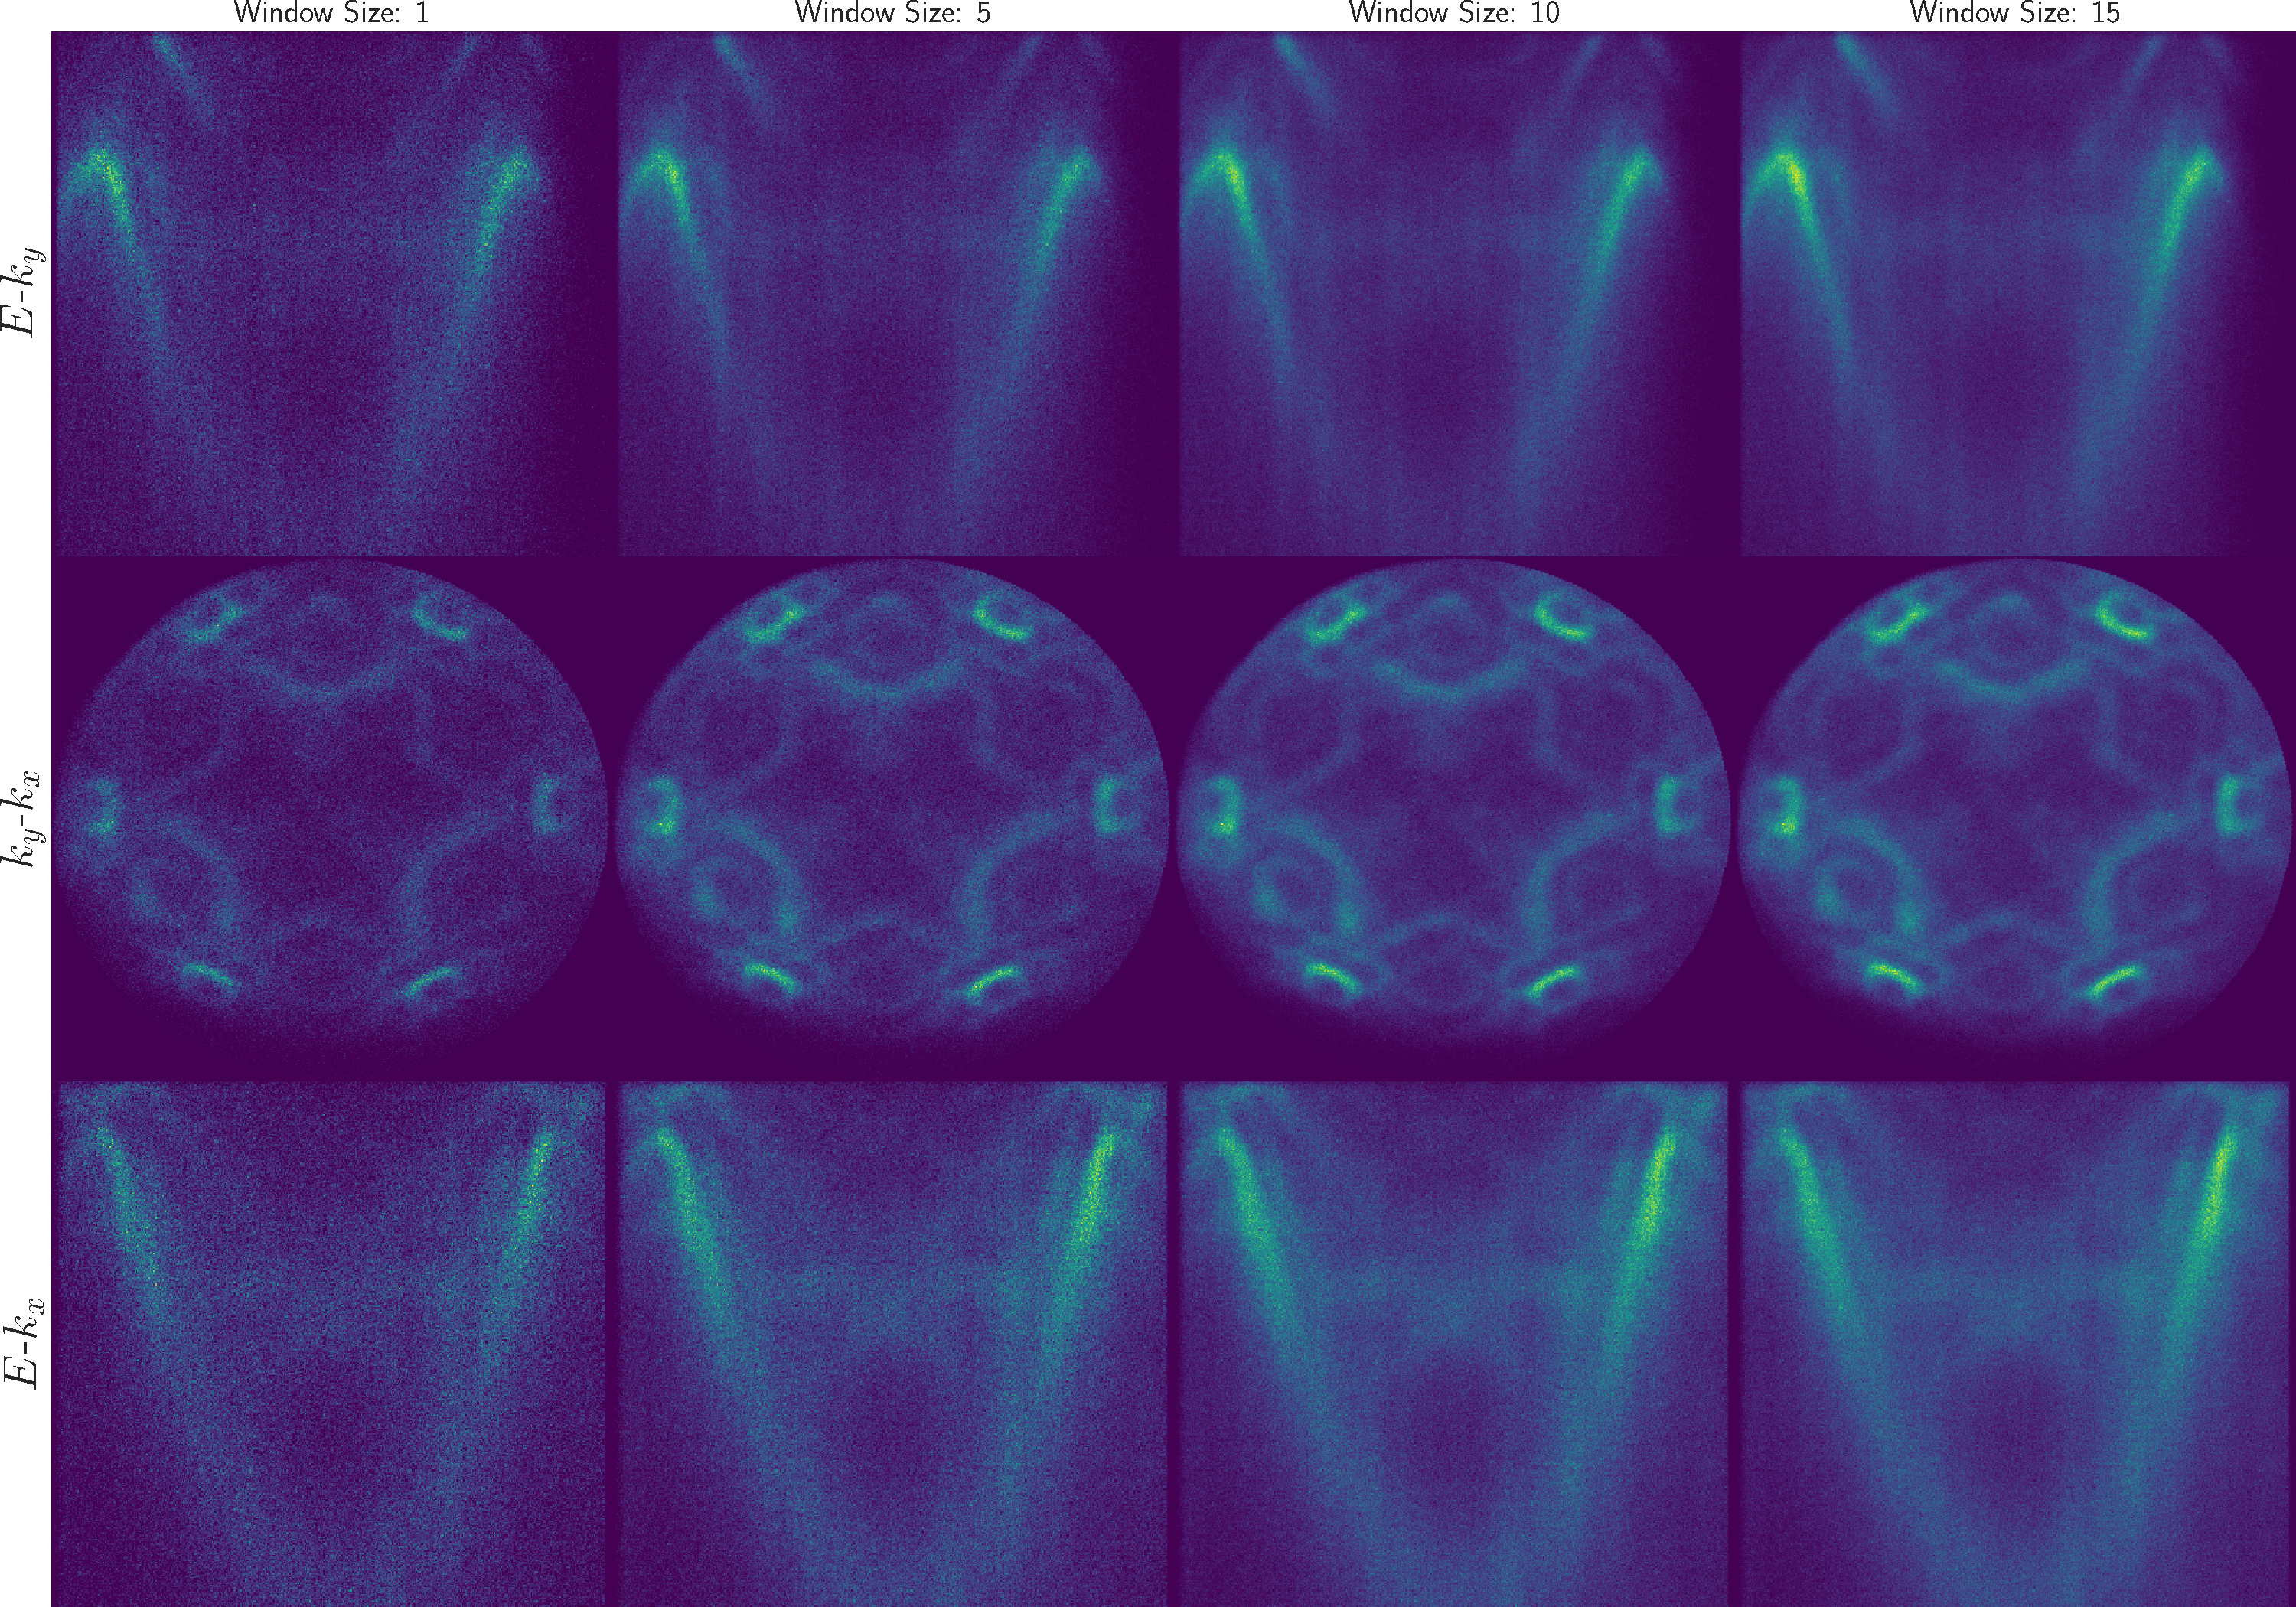
\includegraphics[width=1\linewidth]{images/slices.pdf}
    \caption{2D $E$-$k_x$ images formed from the 3D dataset. The left, middle and right images correspond to a single, average of 5 and average of 10 slices respectively. It can be seen that the noise is reduced, but the features blurred (broadened).}
    \label{fig:slices}
\end{figure}

For evaluation, the images are always normalized as of interest are the relative intensities in the image. The denoising is performed on the 2D slices of the 3D image. The denoised slices are then compared to the true slices using the metrics described above. The results are shown in the next chapter.
